\chapter{Standard for defining $\mu$C Software Store compatible microcontroller based devices}
\label{microcontroller_standard}
\section{Introduction}
This document contains a standard for how microcontroller based devices is identified, and how this makes it possible to filter applications by compatible/incompatible in $\mu$C Software Store. It also defines certain requirements to the wiring of specific components.

All apps that will show up in the $\mu$C Software Store needs to be registered. This is done by sending an application to the management along with the microcontroller app, a wiring diagram and information about the components used.

\section{Basics}
When a $\mu$C-application is registered in the $\mu$C Software Store database, it will have a serial number on eight groups of four hexadecimal digits separated by colons, for example: \textit{2F32:GSE2:F3S3:T32S:G443:45SN:K49D:03J2}. Every registered microcontroller also require having a wiring diagram (schema). Example in Figure~\ref{fig:wiring_simple}:

\begin{figure}[H]
\caption{Example of a wiring diagram (scheme)}
\centering
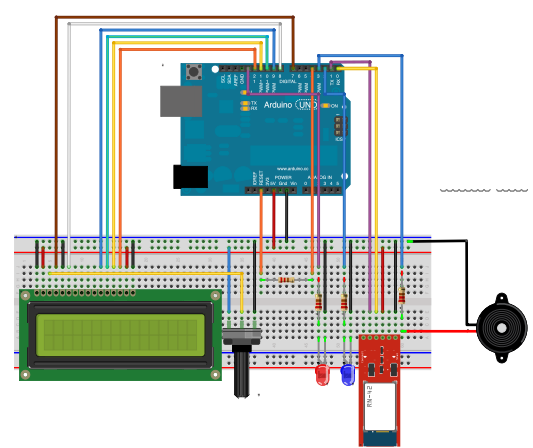
\includegraphics[scale=0.8]{images/wiring_diagram.png}
\label{fig:wiring_simple}
\end{figure}

All components used needs to be registered with the correct model number and the name of the producer, see Table~\ref{table:example_info_xml}\\

\begin{table}[H]
\caption{Example of component information XML document}
\label{table:example_info_xml}
\begin{tabularx}\linewidth{|m{0.33 \textwidth}|X|X|}
	\hline
		{\textbf{Category}} & {\textbf{Model}} & {\textbf{Producer}} \\
	\hline
		{Screen} & {LCD-0025} & {SparkFun} \\
	\hline
\end{tabularx}
\end{table}

In addition, a list of the component pins and which pins these are connected to on the device is required, like in the following example in Table~\ref{table:example_pin_setup}:

\begin{table}[H]
\caption{Example of pin-setup-XML document}
\label{table:example_pin_setup}
	\begin{tabularx}\linewidth{|m{0.5 \textwidth}|X|}
		\hline
			{\textbf{Component pin}} & {\textbf{Device pin}} \\
		\hline
			{0} & {6} \\
		\hline
			{1} & {7} \\
		\hline
	\end{tabularx}
\end{table}

\section{Technical}
The serial number will be stored in the microcontroller`s EEPROM. When a bluetooth connection between the Android application and the microcontroller is established, the serial number is sent from the microcontrollers EEPROM to the Android application. The Android application will lookup the serial number towards a remote database, and retrieve an XML document with information about components and how the pins are connected. If the microcontroller does not have a serial number, or the serial number does not exist in the remote database, no application filtering can be performed.\\ \\

This XML document will be converted to an object that is easier to handle. Every $\mu$C application in the database also has a corresponding XML document that is also converted to an object. This second XML document contains the requirements for the application; for each device mentioned, it will be specified whether this requirement is absolute or not. Apart from this they are identical in structure.\\ \\

When the user clicks on “hide incompatible” the application will filter away (hide) the $\mu$C apps that have more features than the currently connected microcontroller can offer (if a conflicting pin-setup can’t be automatically resolved, this will also happen).\\

\section{Example}
This is the connected device with serial number as shown in Table~\ref{table:serialnr}:\\

\begin{table}[H]
\caption{Serial number to connected microcontroller}
\label{table:serialnr}
	\begin{tabularx}\linewidth{|X|}
		\hline
			{REGR:3T2A:345D:9999:FDHG:53FD:6Y5Y:3FDS} \\
		\hline
	\end{tabularx}
\end{table}

> Doing an XML lookup to remote database and retrieving the XML that belongs to the connected device.
Table~\ref{table:currconnecteddevice} shows the XML for current connected device:

\begin{table}[H]
\caption{The XML document for current connected device}
\label{table:currconnecteddevice}
	\begin{tabularx}\linewidth{|m{0.33 \textwidth}|X|X|}
		\hline
			{\textbf{Category}} & {\textbf{Model}} & {\textbf{Producer}} \\
		\hline
			{} & {Arduino Uno} & {Open Source} \\
		\hline
			{Screen} & {LCD-0025} & {SparkFun} \\
		\hline
			{Red LED} & {COM-09590} & {SparkFun} \\
		\hline
			{BT Module} & {T9J-RN42} & {SparkFun} \\
		\hline
	\end{tabularx}
\end{table}

These (Table~\ref{table:examplerequirement})are the requirements for an example $\mu$C application.

\begin{table}[H]
\caption{he XML document for an example $\mu$C application. The Warn or require field specify whether or not the component has to be present or if the application can run without.}
\label{table:examplerequirement}
	\begin{tabularx}\linewidth{|m{0.25 \textwidth}|X|X|X|}
		\hline
			{\textbf{Category}} & {\textbf{Model}} & {\textbf{Producer}} & {\textbf{Warn or require}} \\
		\hline
			{} & {Arduino Uno} & {Open Source} & {} \\
		\hline
			{Screen} & {LCD-0025} & {SparkFun} & {Require} \\
		\hline
			{Red LED} & {COM-09590} & {SparkFun} & {Warn} \\
		\hline
			{Green LED} & {COM-09592} & {SparkFun} & {Warn} \\
		\hline
			{BT Module} & {T9J-RN42} & {SparkFun} & {Require} \\
		\hline
			{Speaker} & {COM-09151} & {SparkFun} & {Warn} \\
		\hline
			{Potentiometer} & {U-103} & {Sharma} & {Require} \\
		\hline
	\end{tabularx}
\end{table}

> The user selects ``hide incompatible''.

The system (Android application) is doing a check of which applications should be hidden/visible as illutrated in Table~\ref{table:comparasion}:

\definecolor{LightGreen}{RGB}{144,238,144}
\definecolor{LightCoral}{RGB}{240,128,128}

\begin{table}[H]
\caption{Comparison between two XML objects}
\label{table:comparasion}
	\begin{tabularx}\linewidth{|m{0.25 \textwidth}|X|X|X|}
		\hline
			{\textbf{Connected Device}} & {} & {\textbf{Example $\mu$C app}} & {} \\
		\hline
			{\textbf{Model}} & {\textbf{Producer}} & {\textbf{Model}} & {\textbf{Producer}} \\
		\hline
		\rowcolor{LightGreen}
			{Arduino Uno} & {Open Source} & {Arduino Uno} & {Open Source} \\
		\hline
		\rowcolor{LightGreen}
			{LCD-0025} & {SparkFun} & {LCD-0025} & {SparkFun} \\
		\hline
		\rowcolor{LightGreen}
			{COM-09590} & {SparkFun} & {COM-09590} & {SparkFun} \\
		\hline
		\rowcolor{LightGreen}
			{T9J-RN42} & {SparkFun} & {T9J-RN42} & {SparkFun} \\
		\hline
		\rowcolor{LightCoral}
			{COM-09592} & {SparkFun} & {?} & {?} \\
		\hline
		\rowcolor{LightCoral}
			{COM-09151} & {SparkFun} & {?} & {?} \\
		\hline
		\rowcolor{LightCoral}
			{U-103} & {Sharma} & {?} & {?} \\
		\hline
	\end{tabularx}
\end{table}

> Example $\mu$C application will be hidden because it requires more functionality than the current connected microcontroller can offer.
